% !TEX encoding = UTF-8 Unicode
% ÄÖÜ ß äöü

\section{Architecture}

The general design of Ny$\bar{a}$ya follows the Model-View-Controller pattern,
which is originated in Smalltalk \cite[p.4]{GAMMAETAL}, 
that separates the representation of data from the user interaction.
Cocoa Touch \seeref{sec:Cocoa} encourages the use of MVC by providing a rich set of useful views and controllers.
Those cover many use cases of data presentation and user interaction.

\section{Model}

Ny$\bar{a}$ya must hold different representations of Boolean functions – propositional formulas, abstract syntax trees and binary decision diagrams. 

\subsection{Formulas}
Propositional formulas and Boolean expressions are subsets of the set of all Unicode strings. 
Therefore they are easily represented by the standard string class of Cocoa. 

Due to the unambiguous relationship between propositional formulas and Boolean expressions 
Ny$\bar{a}$ya allows the use of a mixed syntax and additional symbols as input
for the user's convenience. The input expression $!a \wedge b + c \oplus a$ translates into the propositional formula
$\neg a \wedge b \vee c \veebar a$.

\subsection{Abstract Syntax Trees}

Cocoa does not provide a class to represent trees, 
but with instances of a class, 
that implements the composite pattern \cite[p.163ff]{GAMMAETAL}
arbitrary graphs and therefore syntax trees can be represented easily.

\begin{figure}[htbp]
\begin{center}
\UML{NyayaNode.png}
\caption{node class to represent an abstract syntax tree}
\label{fig:NyayaNodeCluster}
\end{center}
\end{figure}

\subsubsection{Node class cluster}

The node class is implemented as a class cluster, 
which is an Cocoa design pattern \cite[p.282ff]{Buck:2009:CDP:1803585}
– an adaption of the the abstract factory design pattern \cite[p.87ff]{GAMMAETAL}.
The abstract and public class \verb+NyayaNode+ 
provides a set of static and public methods (see \figref{fig:NyayaNodeCreation}),
that returns instances of non public sub-classes (see \figref{fig:NyayaNodeCluster})
of \verb+NyayaNode+.

\begin{figure}[htbp]
\begin{center}
\UML{NyayaNodeCluster.png}
\caption{public root class and non public subclasses}
\label{fig:NyayaNodeCluster}
\end{center}
\end{figure}

Actual the creational methods are implemented as a class category, 
which is a language feature of Objective-C \cite[p.225ff]{Kochan:2009:PO:1538451}
– an adaption of the decorator design pattern \cite[p.175ff]{GAMMAETAL} –
for extending the functionality of the node class beyond representing a tree. 
There is a standard implementation of the category methods in the root class,
that will be overridden in subclasses.
For example \verb+isLiteral:bool+ returns false for the root class, and all classes but the variable node
and the negation node, when it's child node is a variable node.
The variable node adds setters for some class attributes (see \figref{fig:NyayaNodeValuation}).

\subsubsection{Node class categories}

\begin{itemize}

\item The category “Creation” implements the production rules of the grammar 
to create syntax trees recursively (\figref{fig:NyayaNodeCreation}).
Since the constructors of all classes in the cluster are hidden, 
the production of invalid syntax trees is prevented.

\item The category “Description” provides methods to convert a syntax tree into one of it's string representations – 
either a propositional formula either in strict syntax with many parentheses 
or in a usually shorter formula using precedences and associativity. 

\item The category “Attributes”  provides information about the number of sub-nodes of a node 
and the normal forms the sub-tree matches.

\item The category “Derivations” defines methods to derive semantically equivalent normal forms.

\item The category “Transformations” creates new syntax trees by replacing atoms, connectives or sub-trees with
atoms, connectives or trees.

\item The category “Random” creates arbitrary syntax trees with a given set of connectives and atoms and within a range for the number of nodes. It is used to create formulas for the exercises.

%\item The category “Reductions”
%\item The category “Resolution”
%\item The category “Type”

\begin{figure}[htbp]
\begin{center}
\UML{NyayaNodeValuation.png}
\caption{Valuation of trees}
\label{fig:NyayaNodeValuation}
\end{center}
\end{figure}

\item The category “Valuation” (\figref{fig:NyayaNodeValuation}) 
provides fast valuations with complete truth assignments to create truth tables and binary decision trees. 

\item The category “Display”  allows extended valuations with incomplete truth assignments. 
It is used in the SyntaxTreeView, where the user can assign truth values to some or all atoms.
% (see \figref{fig:NyayaNodeDisplay)
\end{itemize}

\subsubsection{Syntactical Immutability}

\begin{figure}[htbp]
\begin{center}
\UML{NyayaNodeCreation.png}
\caption{Production rules}
\label{fig:NyayaNodeCreation}
\end{center}
\end{figure}

Regarding their function as syntax tree nodes instances of the node class are not mutable. 
Node instances can be created (\figref{fig:NyayaNodeCreation}), but not modified.
The symbol of an atom can not be changed, 
a connective can not be altered into an other one,
the arguments of a connective can not be replaced or reordered.
Derivations or transformations do not change the structure of an existing syntax tree,
but rather create a new independent syntax tree.

Obviously mutable truth assignments does not affect the immutable structure of a syntax tree,
because truth assignments are semantics, not syntax. 

\subsubsection{Runtime representation}

Since the representation of abstract syntax tress in Ny$\bar{a}$ya is designed immutable,
there is no need to create multiple instances for syntactically equivalent sub-trees. 
At run-time syntax trees are represented by acyclic directed graphs, 
where multiple sub-trees can be represented by the same object-graph
(\figref{fig:AcyclicSyntaxGraph}).

\begin{figure}[htbp]
\begin{center}
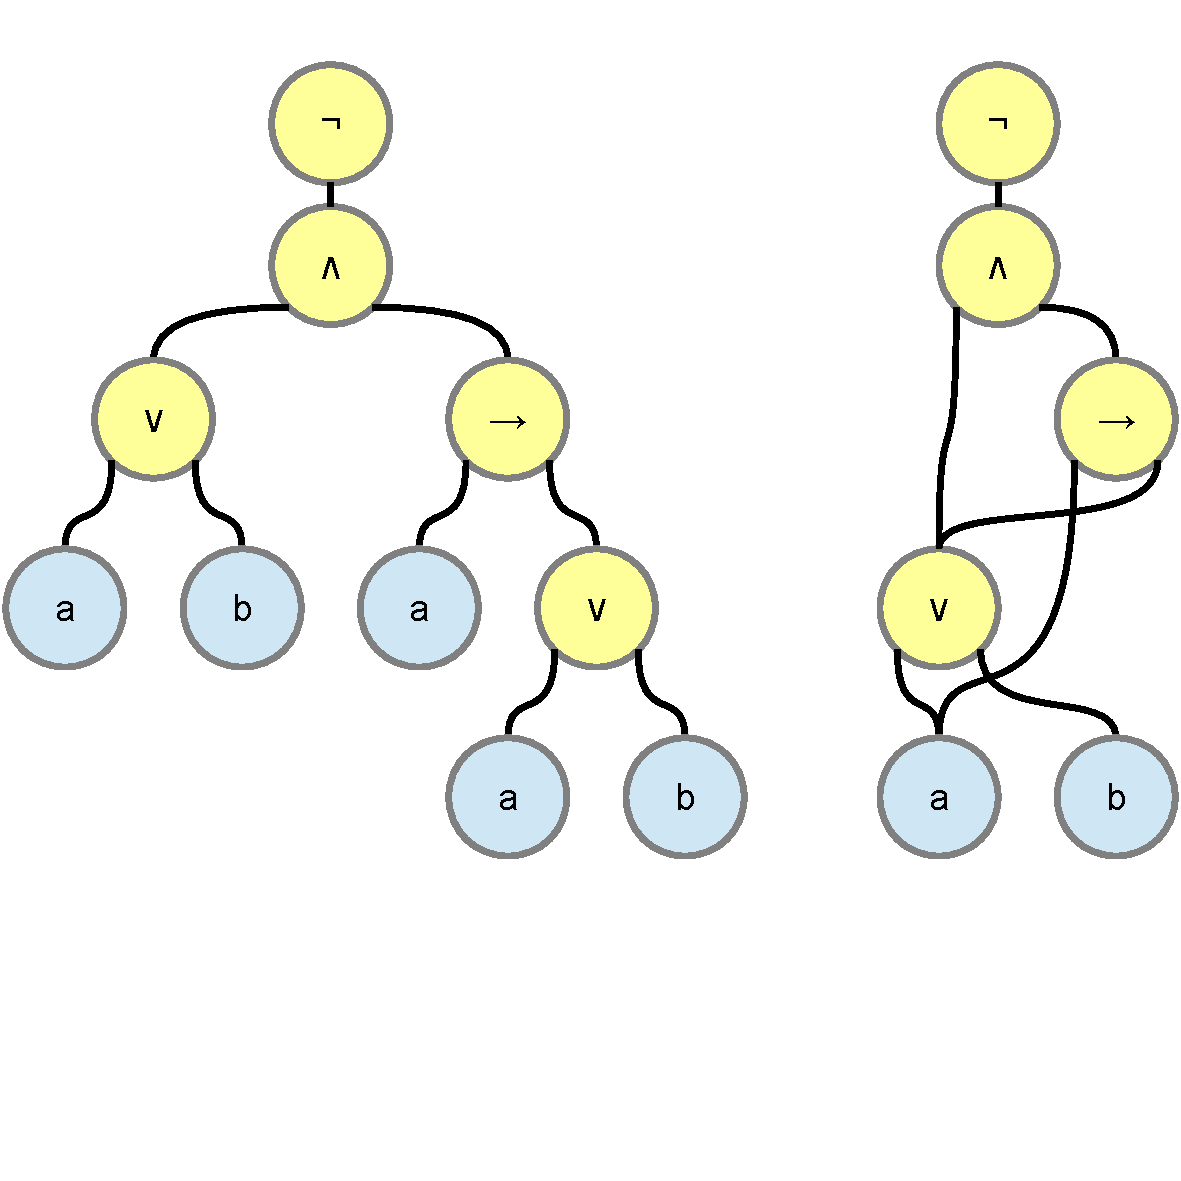
\includegraphics[scale=0.5,trim=0cm 2.9cm 0cm 1cm,clip=true]{diagrams/AcyclicSyntaxGraph.pdf}
\caption{Abstract syntax tree and runtime representation}
\label{fig:AcyclicSyntaxGraph}
\end{center}
\end{figure}

This eases the detection of obvious tautologies $P \vee \neg P$, $P \rightarrow P$ and contradictions $P \wedge \neg P$,
because the sub-tree $P$ on the left side is represented by the same object-graph as the sub-tree $P$ on the right side.

\subsection{Binary Decision Diagrams}

Binary decision trees and diagrams are represented by trees or acyclic directed graphs built from instances of a simple class
\begin{table}[htdp]
\begin{center}
\UML{BddNode.png}
\caption{Public attributes and factory method of BddNode}
\label{fig:BddNode}
\end{center}
\end{table}
 with a name, a left branch and a right branch. The name is either an identifier (name of a variable), “0” or “1". 
Nodes with the name “0” or “1” are leaf nodes and therefore must not have a left or right branch.
The other nodes must have valid left and right branches. The class provides factory method(s) to create 
(reduced, ordered) binary decision diagrams from representations of Boolean functions
(\figref{fig:BddNode}).


\subsection{Parser}

The backend of \verb+BoolTool+\footnote{
\href{http://cl-informatik.uibk.ac.at/software/booltool/}{cl-informatik.uibk.ac.at/software/booltool/}} 
– parsing and transformation of Boolean functions – 
is implemented in \verb+OCaml+\footnote{
\href{http://ocaml.org}{ocaml.org}}, 
a functional programming language, which is well suited for this kind of task.

After several failed attempts to cross-compile the \verb+OCaml+ sources to iPad's processor architecture (ARM),
to link the object code to the Xcode project and to bridge and call functions from C, 
the implementation of a simple translator 
for propositional formulas (a subset of all possible strings)
into syntax trees looked more promising. 
This was achieved by using standard techniques of compiler construction \cite{Louden:1997:CCP:523017}. 

\subsubsection{Scanning}

\begin{table}[htdp]
\begin{center}
$\top | \bot 
| \neg | !
| \wedge | \& | .
| \vee | {\setminus}| | {\setminus}+ 
| \veebar | \oplus | \textasciicircum
| = | <> | \leftrightarrow 
| > | \rightarrow | \models
| ( | ) | , | ; 
| {\setminus}w+$ 
\caption{Regular expression for the lexxer of Ny$\bar{a}$ya}
\label{tab:REGEX}
\end{center}
\end{table}
The set of valid tokens (identifiers, connectives and parentheses) 
is defined by a regular expression (\tabref{tab:REGEX}). 
In the first step of translating a propositional formula,
the input string is transformed into an array of strings 
using the standard regular expression class of Cocoa Foundation.

\subsubsection{Parsing}
\begin{table}[htdp]
\begin{center}
\begin{lstlisting}[mathescape]
formula        ::= entailment
entailment     ::= sequence [ $\models$ entailment]
sequence       ::= bicondition { ; bicondition } 
bicondition    ::= implication [ $\leftrightarrow$ bicondition ]
implication    ::= xdisjunction [ $ \rightarrow$ implication ]
xdisjunction   ::= disjunction { $\veebar$ disjunction }
disjunction    ::= conjunction { $\vee$ conjunction }
conjunction    ::= negation { $\wedge$ negation }
negation       ::= $\neg$ negation | ( formula ) | identifier
\end{lstlisting}
\caption{EBNF grammer for the parser of Ny$\bar{a}$ya}
\label{tab:EBNF}
\end{center}
\end{table}


\section{Views}

\begin{figure}[htbp]
\begin{center}
\UML{TreeView.png}
\caption{Tree viewr}
\label{fig:TreeView}
\end{center}
\end{figure}

\begin{figure}[htbp]
\begin{center}
\UML{NyayaNodeDisplay.png}
\caption{Node display interface}
\label{fig:NyayaNodeDisplay}
\end{center}
\end{figure}

\section{Controllers}








\section{Unit-Tests}

\section{Content}



